\documentclass{article}

%%% packages %%%%%%%%%%%%%%%%%%%%%%%%%%%%%%%%%%%%%%%%%%%%%%%%

%-- page setup ----------------------------------------------

\usepackage[utf8]{inputenc}
\usepackage[a4paper, margin=1in]{geometry}

%-- font ----------------------------------------------------

\usepackage[T1]{fontenc}

%-- img ---------------------------------------------------------

\usepackage{graphicx}

%-- head/foot -----------------------------------------------

\usepackage{fancyhdr}

\pagestyle{fancy}

\fancyhead[l]{Vincent von Schmidt\\Niklas Zock}
\fancyhead[c]{L17 - Informatik}
\fancyhead[R]{\today}

\renewcommand{\footrulewidth}{0.4pt}
\fancyfoot{}
\fancyfoot[L]{Software - Projekt\\Mini Chess}
\fancyfoot[R]{\thepage}

%------------------------------------------------------------
%%%%%%%%%%%%%%%%%%%%%%%%%%%%%%%%%%%%%%%%%%%%%%%%%%%%%%%%%%%%%

\title{\textbf{Software - Projekt\\Mini Chess}}
\date{\vspace{-5ex}}

\begin{document}

\maketitle
\thispagestyle{fancy}

%%% content %%%%%%%%%%%%%%%%%%%%%%%%%%%%%%%%%%%%%%%%%%%%%%%%%

\tableofcontents
\newpage

%------------------------------------------------------------

\section{Ziele}\label{section-goals}

\subsection{Minimalanforderung}
\begin{itemize}
    \item simple Oberfläche -> start via cmd
    \item rating algo
    \item 3x3
    \item PyQt GUI
\end{itemize}

\subsection{Zusatzanforderung}
\begin{itemize}
    \item 4x4; 5x5
    \item PyQt embeded pygame $\rightarrow$ für bessere Effizent
\end{itemize}

%------------------------------------------------------------

\newpage
\section{Systemanforderung}\label{section-requirements}

\subsection{Hardware}
\begin{itemize}
    \item 8 GB RAM
    \item 32 MB Speicher
    \item Maus und Tastatur
    \item Farbbildschirm (empfohlen)
\end{itemize}

\subsection{Software}
\begin{enumerate}
    \item Ausführen via .exe $\rightarrow$ Windows 10 21H2 +
    \item Ausführen via Python
        \begin{itemize}
            \item Python 3.11+ $\rightarrow$ Python 3.11 für bessere Effizents
            \item Python libarys $\rightarrow$ einfacher Installationsprozess via requirements.txt
                \begin{itemize}
                    \item PyQt6
                    \item pygame 2.4
                \end{itemize}
        \end{itemize}
\end{enumerate}

\subsection{Merkmale}
\begin{center}
    sehr großer Fokus: ++    großer Fokus: +    mittlerer Fokus: o    kleiner Fokus: -    sehr kleiner Fokus: --
    \begin{tabular}{ |c|c| }
        \hline
        Merkmale & Gewichtung \\
        \hline
        & Benutzerfreundlichkeit & ++ \\
        \hline
        & Korrektheit & + \\
        \hline
        & Wartungsfreundlichkeit & + \\
        \hline
        & Zuverlässigkeit & ++ \\
        \hline
        & Effizienz & o \\
        \hline
    \end{tabular}
\end{center}


%------------------------------------------------------------

\newpage
\section{Produktumgebung}\label{section-product}

\subsection{Benutzeroberfläche}

\begin{figure}[h]
    \centering
    \fbox{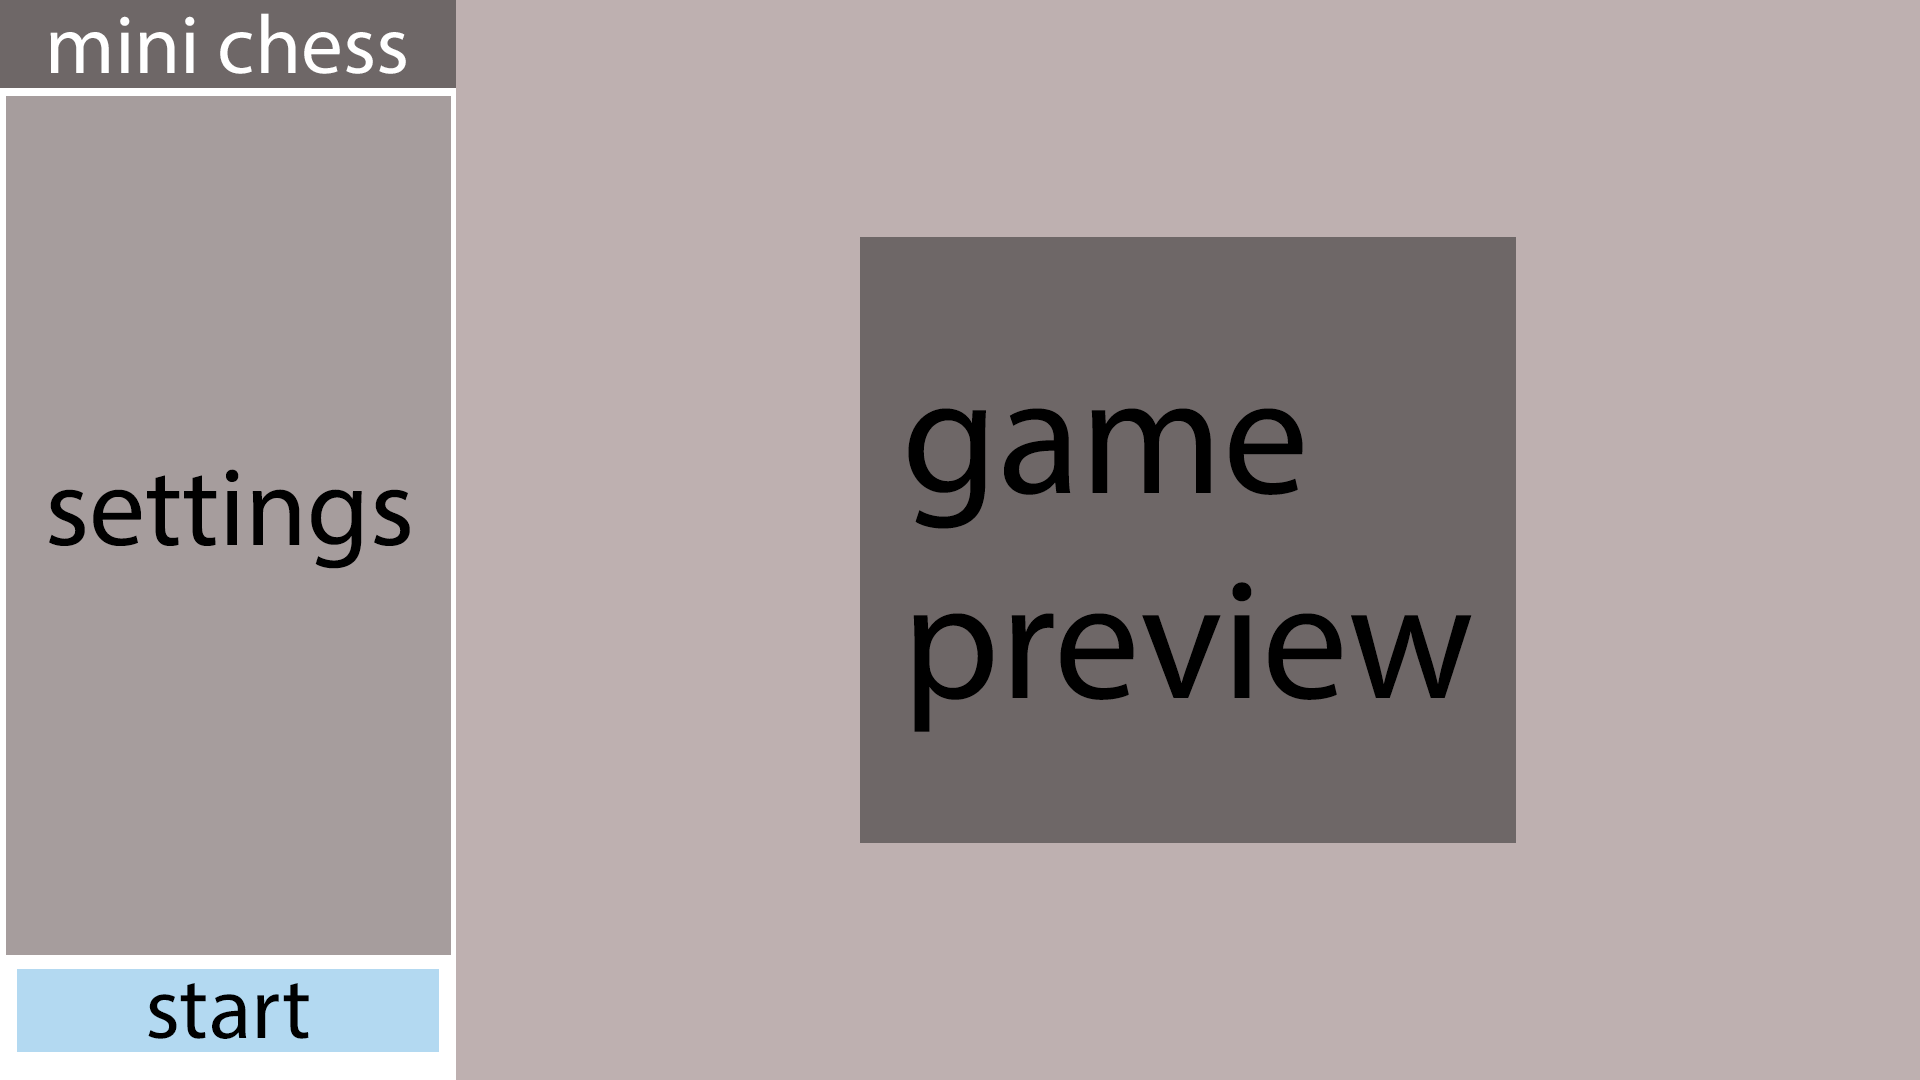
\includegraphics[width=\textwidth, keepaspectratio]{gui_conzept_start_screen.png}}
    % \caption{Startscreen}
\end{figure}

\begin{figure}[h]
    \centering
    \fbox{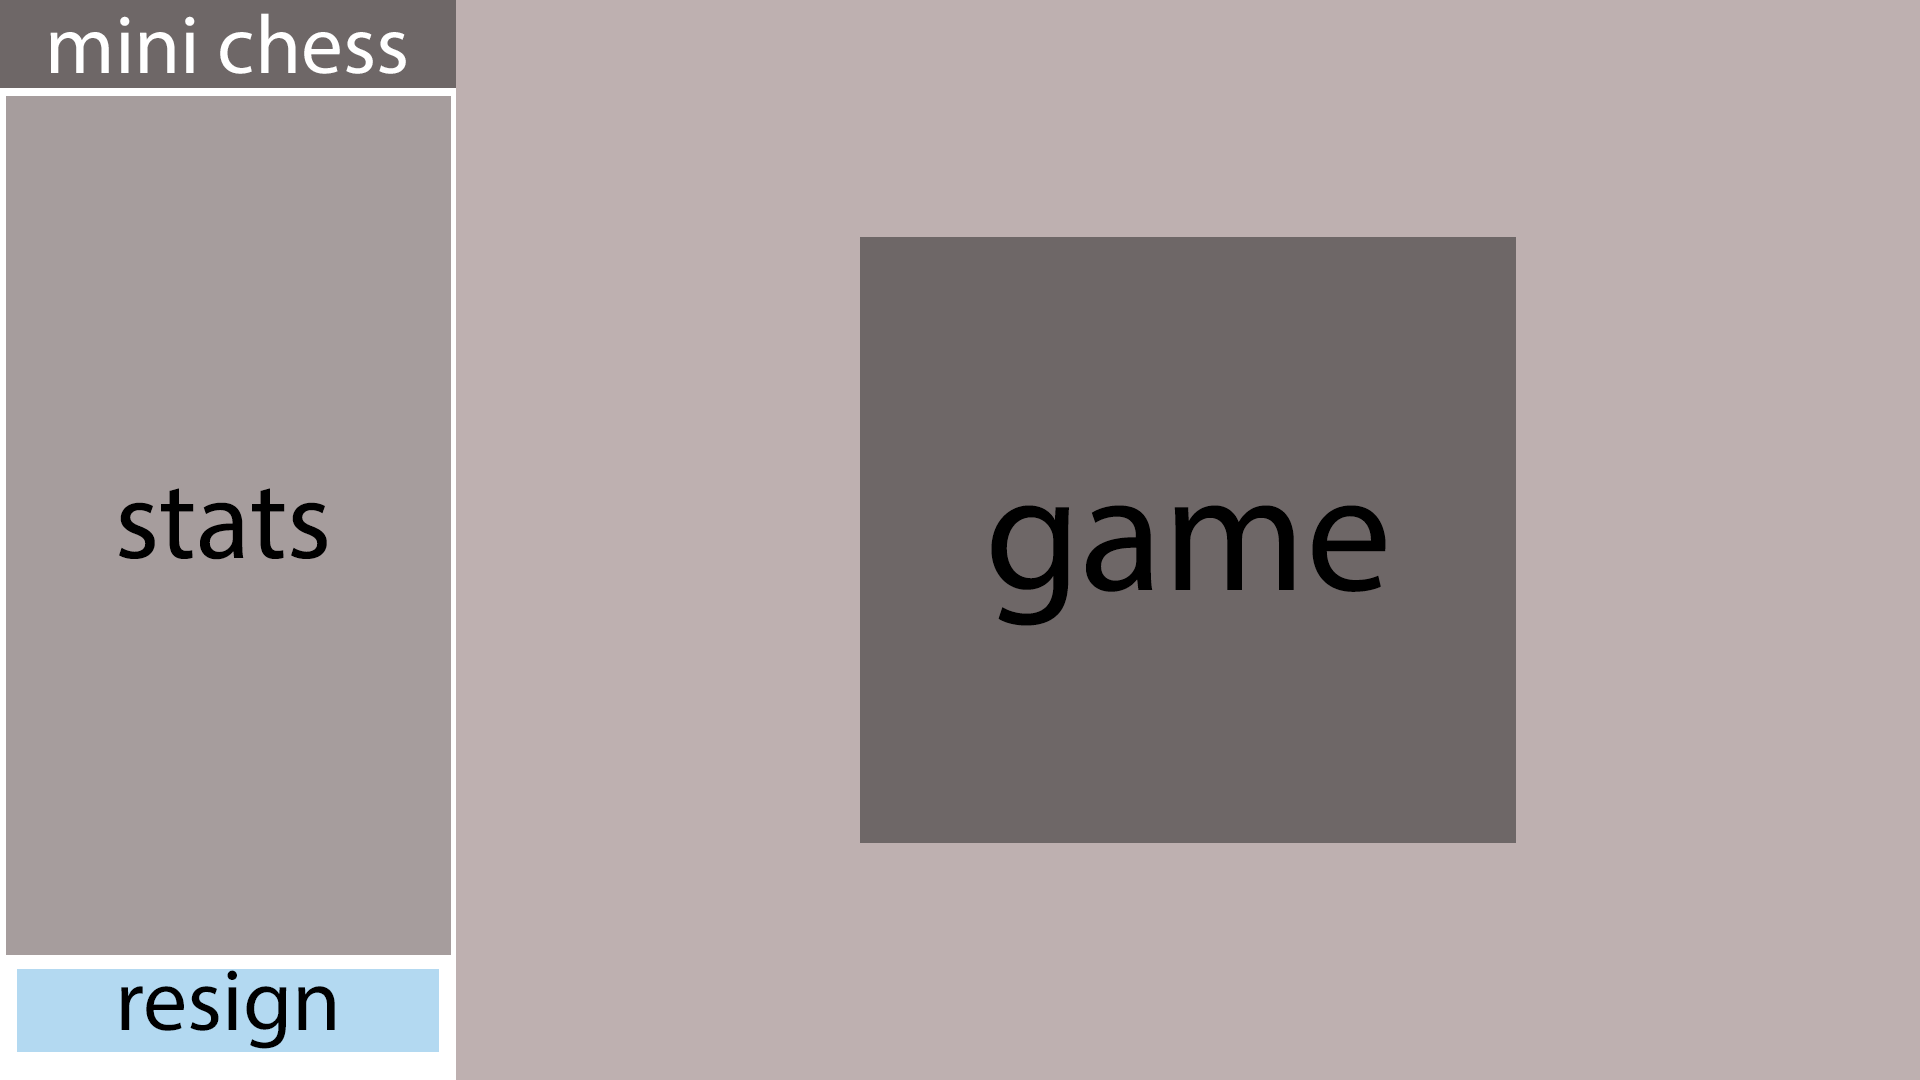
\includegraphics[width=\textwidth, keepaspectratio]{gui_conzept_game_screen.png}}
    % \caption{Gamescreen}
\end{figure}

\subsection{Klasendiagramm}
\subsection{Spezifikationen}

%------------------------------------------------------------

\newpage
\section{Arbeitstagebuch}\label{section-diary}

\subsection{Chronologie}
\subsection{Testläufe}

%------------------------------------------------------------

%%%%%%%%%%%%%%%%%%%%%%%%%%%%%%%%%%%%%%%%%%%%%%%%%%%%%%%%%%%%%

\end{document}
